\section{Experiments}
%\subsection{Experimental Setup}
%\textbf{Dataset and Evaluation Methodology}. 
We use Freebase and the English Wikipedia dump of 2016-11-20, to construct our dataset. Statistics for the generated dataset from Freebase is shown in Table~\ref{statistics}. Note that we only include positive sentences in this dataset. 
\begin{table}
\small
\centering
\begin{tabular}{|l|c|c|c|} \hline
& Train & Dev & Test \\ \hline
\emph{\#PosSent.} & 29912 & 7477 & 9346 \\ \hline
\emph{\#NegSent.} & 50904 & 12726 & 15906  \\ \hline
\emph{\#Eve.} &  &  &  \\ \hline
\emph{\#Arg.} &  &  &  \\ \hline
\emph{\%Multi\_Eve.} &  &  &  \\ \hline
\end{tabular}
\caption{Statistics for the generated dataset. \emph{\#PosSent.} is the number of positive sentences, \emph{\#NegSent.} is the number of positive sentences, \emph{\#Eve.} is the number of event mentions, and \emph{\#Arg.} is the number of event arguments. \emph{\%Multi\_Eve.} is the ratio of multi-type events.
%, and \emph{\%Multi\_Arg.} is the ratio of multi-word arguments.
\label{statistics}}
\end{table}

% containing 7,180 sentences, containing 7,394 events and 25,840 arguments. We then randomly select 4,800 sentences for training and 1,180 sentences as test set, and the rest 1,200 sentences for validation. 
We first manually evaluate the quality of our test set and then regard the automatically generated data as gold standard and evaluate our model accordingly. Next, we manually evaluate a subset of events detected by our model and analyze the differences with regards to the automatic evaluation. Finally, we conduct evaluation on a smaller dataset constructed according to Wikipedia tables and articles. 

\paragraph{Evaluation Metrics:} We evaluate our models in terms of precision (P), recall (R), and F-measure (F) for each subtask. These metrics are computed according to the following standards of correctness: 
For \emph{event type classification}, an event is correctly classified if its reference sentence contains \textbf{all key arguments} of this event type. 
For \emph{event detection}, an event is correctly detected if its type and all its key arguments match a reference event within the same sentence.
For \emph{argument detection}, an argument is correctly detected if its offsets, role, and related event type exactly match the reference argument within the same sentence. 

\paragraph{Training:} All hyper-parameters are tuned on the development set. During event detection, we set the size of word embeddings to 200, the size of LSTM layer to 100. In argument detection, we use the same size of word embedding, while the size of LSTM layer is 150, and the size of key argument embedding is 50. Word embeddings are pre-trained using skip-gram word2vec~\cite{mikolov2013distributed} on English Wikipedia and fine tuned during training. We apply dropout (0.5) on both input and output layers.

% TODO: 介绍如何抽样构造负例
\paragraph{Negative samples:} 

\subsection{Dataset Evaluation}\label{sec:evalhypo}
To investigate the possibility of automatically constructing training data for event extraction, we evaluate five datasets that utilize  following strategies to determine key arguments and collect positive instances: (1) \emph{ALL} means regarding all arguments as key arguments; (2) \emph{IMP} means selecting the top half arguments with high importance value as key arguments; (3) \emph{IMP\&TIME} means adding a time-related argument with highest importance value to the set of key arguments defined by \emph{IMP}; (4) \emph{DIS} means eliminating sentence where dependency distances between any two key arguments are greater than 2. We randomly select 100 sentences from each dataset, and annotators are asked to determine whether each sentence implies a given event.

\begin{table}[h]
\small
\centering
\begin{tabular}{|c|l|c|c|c|} \hline
	No. & Strategy & Sent. & Type & Post. \\ \hline
	T1 & \emph{ALL} & 203 & 9 & 98\% \\ \hline
	T2 & \emph{IMP} & 108K & 24 & 22\% \\ \hline
	T3 & \emph{IMP}+\emph{DIS} &  &  & 37\% \\ \hline
	T4 & \emph{IMP\&TIME} &  &  & 81\% \\ \hline
	T5 & \emph{IMP\&TIME}+\emph{DIS} &  &  & 89\% \\ \hline
\end{tabular}
\caption{Statistics of the datasets built with different strategies. 
% \textit{Instances} denotes the number of CVT instances that can be used for each hypothesis. 
\textit{Sent.} is the number of found sentences. \textit{Type} the number of different CVT types found within each dataset.  \textit{Post.} is the percent of sentences mentioning the given events explicitly. \label{tab:3}}
\end{table}

As shown in Table~\ref{tab:3}, it is not surprising that the most strict strategy, \emph{T1}, guarantees the quality of the generated data, while we can merely obtain 203 sentences covering 9 types of events, which is insufficient for further applications. \emph{T2} relaxes \emph{T1} by allowing the absence of non-key arguments, which expands the resulting dataset, but introduces more noise, indicating that \emph{T2} is inappropriate to be used as a soft constraint. Compared with \emph{T2}, the significant quality improvement by \emph{T4} proves that time-related arguments within CVT schemas are critical to imply an event occurrence. Among all strategies, data obtained by \emph{T5} achieves the highest precision, while still accounting for 7,180 sentences, showing that it is feasible to automatically collect quality training data for event extraction without either human-designed event schemas or \textbf{extra} human annotations.     
% our hypothesis \emph{H3} and \emph{H4} are feasible and it is an effective way to generate reliable data automatically.

\subsection{Baselines}
%To investigate the effectiveness of our proposed model, 
We compare our proposed models with three baselines, including traditional feature-based methods and neural network models. All baselines are trained following the two-step pipeline, i.e., event detection and argument detection.
For neural network methods, we train a  BLSTM model that takes word embeddings as input, and outputs the label with the maximum probability among all possible labels. 
For feature-based methods, we apply Conditional Random Field \cite{lafferty2001conditional} (with the CRF++ toolkit~\cite{kudo2005crf++} ) and Maximum Entropy \cite{berger1996maximum} (Le Zhang's MaxEnt toolkit) to explore a variety of elaborate features, such as lexical, syntactic and entity-related features, according to the state-of-art feature-based ACE event extraction system~\cite{li2013joint}. Note that during argument detection stage, we add the label of each word output by event detection as a supplementary feature.
%We use Stanford CoreNLP \cite{manning2014stanford} for feature extraction, and utilize the CRF++ toolkit~\cite{kudo2005crf++} and Le Zhang's MaxEnt toolkit \footnote{\url{https://github.com/lzhang10/maxent}} to train the CRF and Max Entropy classifiers, respectively.

\subsection{Automatic Evaluation}
As shown in Table~\ref{tab:1}, traditional feature-based models perform worst in both event detection and argument detection. 
One of the main reasons is the absence of explicit event trigger annotations in our dataset, which makes it impossible to include trigger-related features, e.g., trigger-related dependency features and positions of triggers. 
Although traditional models can achieve higher precisions, they only extract a limited number of events, resulting in low recalls. 
Neural-network methods perform much better than feature-based models, especially recalls, since they can make better use of word semantic features. Specifically, BLSTM can capture longer range dependencies and richer contextual information, instead of neighboring word features only.
And the CRF component brings an averagely 4\% improvement in all metrics, and by adding the ILP-based post inference module, our full model, BLSTM-CRF-ILP$_{multi}$, achieves the best performance among all models. 
% Moreover, neural-network-based methods can avoid errors propagating from other NLP preprocessing tools like POS tagging and NER.

\begin{table*}[!t]
\centering
\small
\begin{tabular}{|l|p{0.8cm}<{\centering}|p{0.8cm}<{\centering}|p{0.8cm}<{\centering}|p{0.8cm}<{\centering}|p{0.8cm}<{\centering}|p{0.8cm}<{\centering}|p{0.8cm}<{\centering}|p{0.8cm}<{\centering}|p{0.8cm}<{\centering}|} \hline
	\multirow{2}{*}{Model} & \multicolumn{3}{c|}{Event Classification} & \multicolumn{3}{c|}{Argument Detection} &
	\multicolumn{3}{c|}{Event Detection} \\ \cline{2-10}
	 & P & R & F & P & R & F & P & R & F \\ \hline
	CRF &  &  &  &  &  &  &  &  &  \\ \hline
	MaxEnt &  &  &  &  &  &  &  &  &  \\ \hline
	BLSTM &  &  &  &  &  &  &  &  &   \\ \hline \hline
	BLSTM-CRF &  &  &  &  &  &  &  &  &   \\ \hline
	BLSTM-CRF-ILP$_{1}$ &  &  &  &  &  &  &  &  &  \\ \hline
	BLSTM-CRF-ILP$_{multi}$ &  &  &  &  &  &  &  &  &  \\ \hline
\end{tabular}
\caption{Overall system performance of automatic evaluations (\%).  \label{tab:1}}
\end{table*}

% \paragraph{Multi-word Argument Detection}
% Committing to the multi-word argument issue, we treat each subtask as a sequence labeling problem. Evaluated on multi-word arguments, the F1 scores of BLSTM-CRF, BLSTM-CRF-ILP$_1$ and BLSTM-CRF-ILP$_{multi}$ in argument detection are 71.3\%, 80.5\%, and 81.0\%, respectively. 

\paragraph{Effect of CRF Layer} 
Every model with a CRF layer over its BLSTM output layer is superior to the one with a BLSTM layer only. Compared with the BLSTM, BLSTM-CRF achieves higher precisions and recalls in all subtasks by significantly reducing the invalid labeling sequences (e.g., \texttt{I-arg} appears right after \texttt{O}). During prediction, instead of tagging each token independently, BLSTM-CRF takes into account the constraints between neighboring labels, and potentially increases the cooccurrences of key arguments regarding the same event type. % in some way. 

\paragraph{Effect of Post Inference} 
As shown in Table~\ref{tab:1}, ILP-based post inference considerably improves the overall system performance, especially in event type classification. With the help of constraint \textbf{C4},  some dubious key arguments can be inferred through other key arguments from their contexts. Compared with BLSTM-CRF, BLSTM-CRF-ILP$_1$ produces an F1 gain of 7.4\% in event type classification, 1.8\% in event detection, and 4.6\% in argument detection. %, with respect to tF1. 

\paragraph{Multi-type Event Extraction}
We further investigate the effect of BLSTM-CRF-ILP$_{multi}$, which is the only model that can deal with the mulit-type event mentions. As shown in Table~\ref{tab:1}, the proposed strategy in BLSTM-CRF-ILP$_{multi}$ helps detect more event mentions, contributing to the increase of recalls, and F1 scores with a little drop of precisions. Evaluated on 38 sentences containing multi-type event mentions, the F1 scores of BLSTM-CRF-ILP$_{multi}$ in event type classification, event detection and argument detection are 70.7\%, 58.4\% and 26.9\%, respectively.

\subsection{Manual Evaluation \label{manualeve}}
We randomly sample 150 sentences from the test set. Annotators are asked to annotate all arguments to each sentence following two steps. First, determine whether a given sentence is positive or negative, and assign event types to positive sentences. Next, label all related arguments and their roles according to the event types for positive sentences. Two annotators will independently annotate each sentence, and discuss to achieve an agreement. The inter-annotator agreement is 87\% for event types and 79\% for arguments.

\begin{table}[h]
\small
\centering
\begin{tabular}{|l|p{0.8cm}<{\centering}|p{0.8cm}<{\centering}|p{0.8cm}<{\centering}|} \hline
	Model & EC & AD & ED \\ \hline
	CRF & 21.2 & 13.3 & 5.30 \\ \hline
	MaxEnt & 17.7 & 11.7 & 5.44 \\ \hline
	BLSTM & 79.8 & 64.3 & 41.2 \\ \hline \hline
	BLSTM-CRF & 81.3 & 67.9 & 43.2 \\ \hline
	BLSTM-CRF-ILP$_{1}$ & 85.0 & 70.4 & 43.8 \\ \hline
	BLSTM-CRF-ILP$_{multi}$ & \textbf{85.3} & \textbf{70.8} & \textbf{44.3} \\ \hline
\end{tabular}
\caption{ The F1 scores of different systems on the manually annotated data. EC, AD, ED denote the event type classification, argument detection and event detection, respectively. \label{tab:2}}
\end{table}

Table~\ref{tab:2} shows the system performances in the manual evaluation. We can draw similar conclusions about the comparison of performances between different models as automatic evaluation. It is clear that BLSTM-CRF-ILP$_{multi}$ is the most effective model in event extraction as it achieves the highest F1 scores in both manual and automatic evaluation.

\begin{figure}[h]
	\centering
	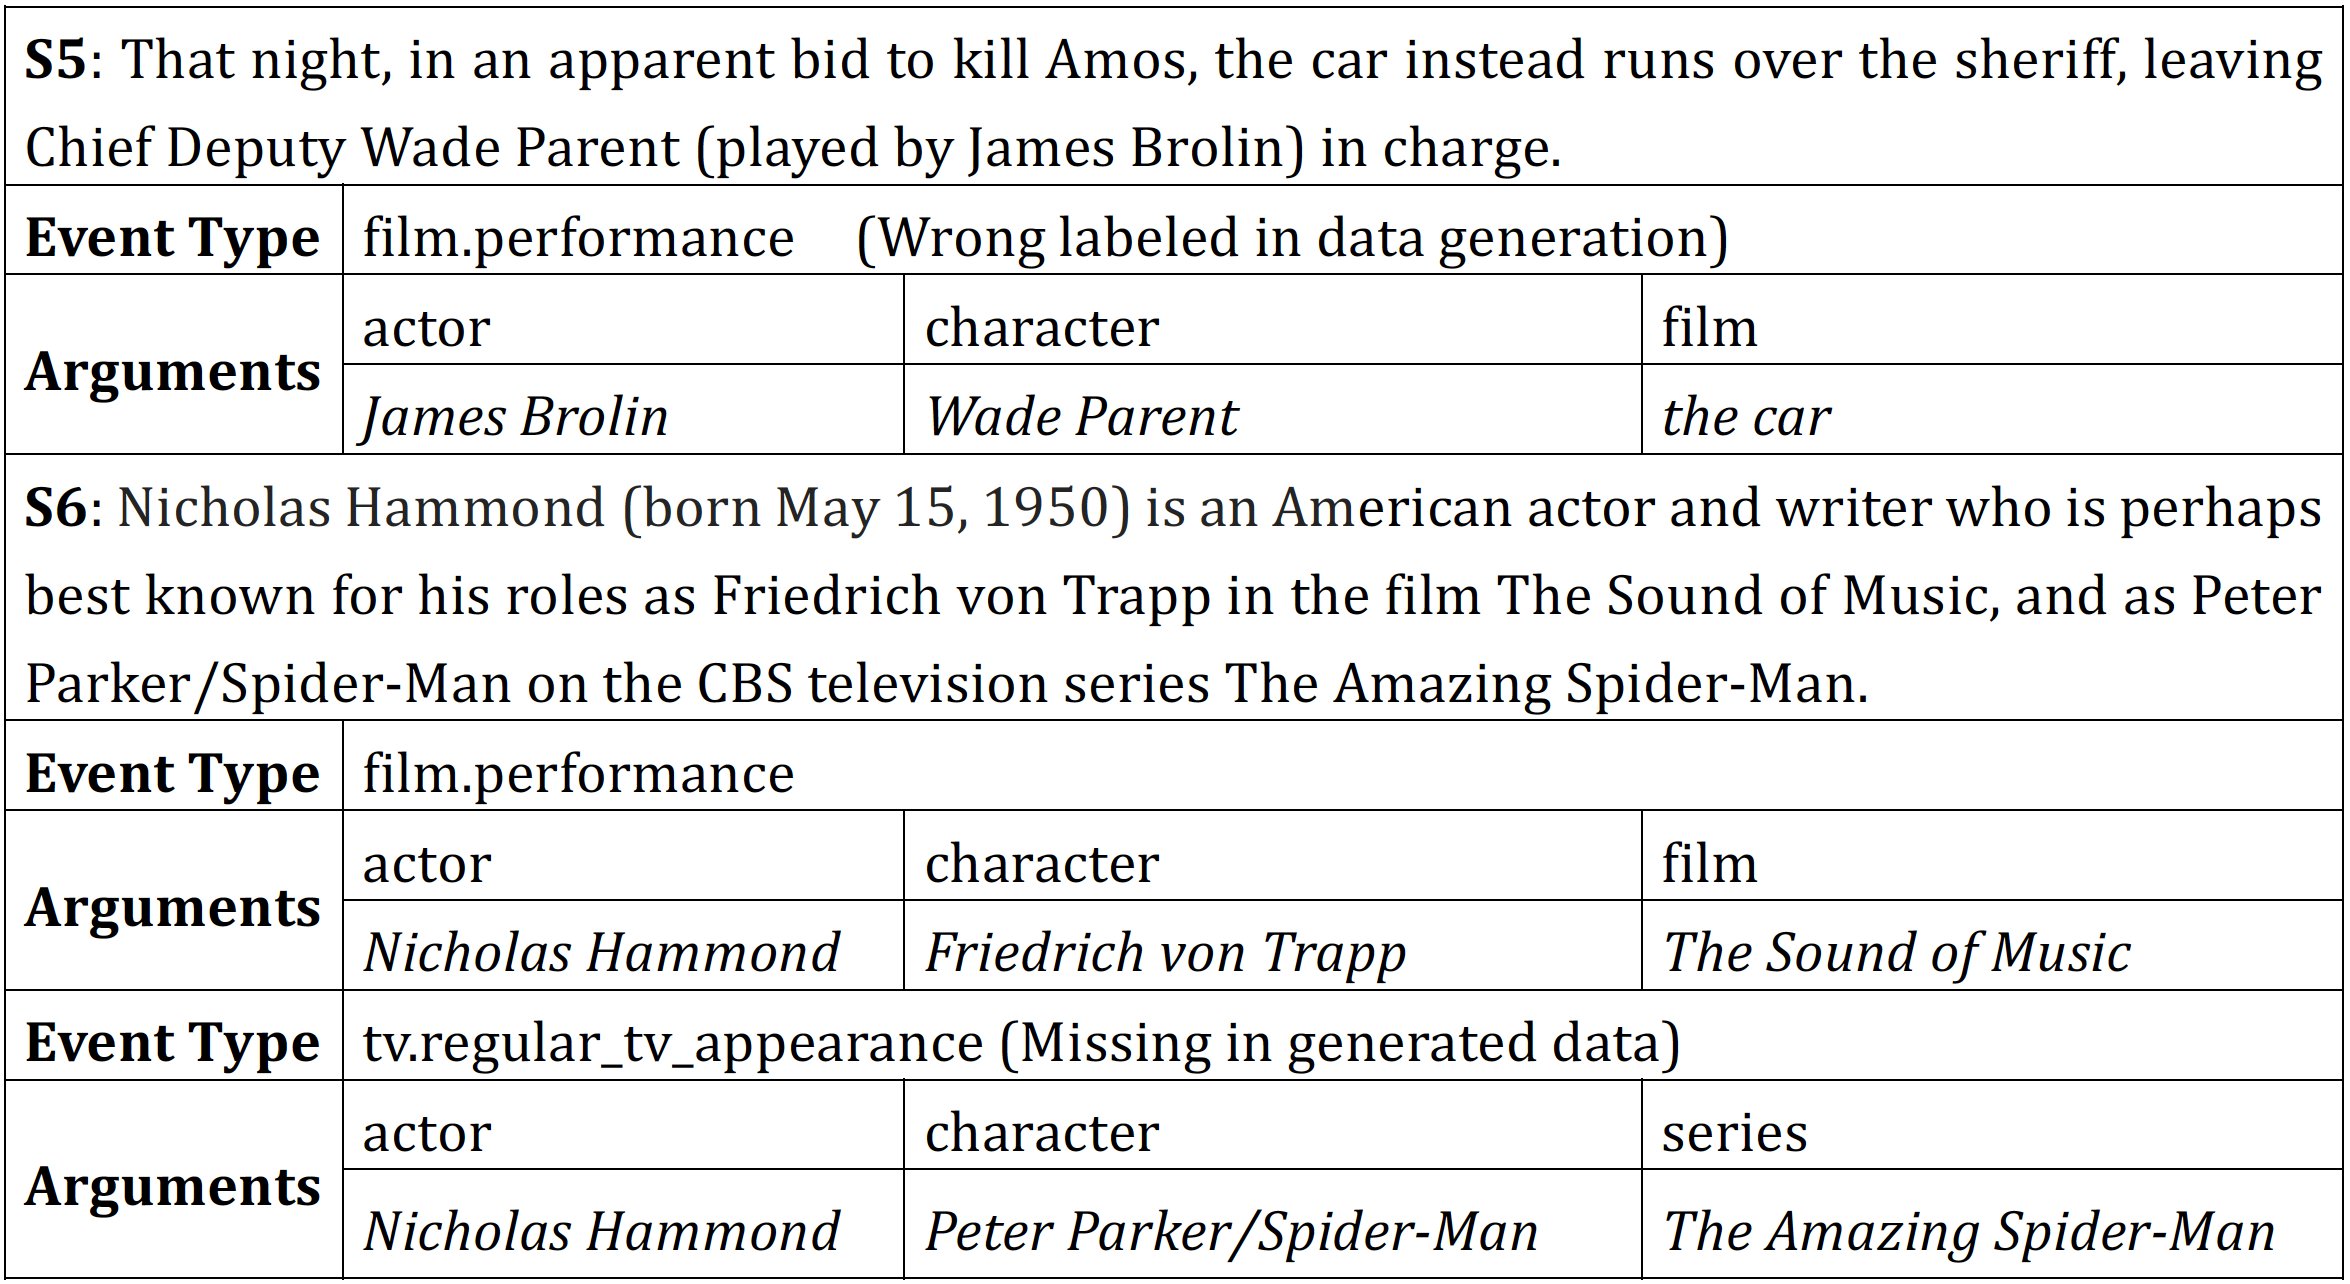
\includegraphics[width=.48\textwidth]{figure3.png}
	\caption{Example outputs of BLSTM-CRF-ILP$_{multi}$.\label{fig:1}}
\end{figure}

Moreover, %manual evaluation may help us to gain a deep insight about our data and models. We 
 we manually check the top 5 event types whose EC F1 scores by BLSTM-CRF-ILP$_{multi}$ differ greatly between automatic evaluation and manual evaluation, summarized in Table~\ref{tab:4}. We find that most of the performance differences are caused by data generation. Figure~\ref{fig:1} examples two types of errors in data construction. Several automatically labeled sentences do not imply any event while still matching all key properties of some CVT entries. For an example, although the phrase \emph{the car} in S5 matches a film name, it does not indicate this film, and there is no explicit evidence indicating that an actor starred in this film. This is a bottleneck of our data generation strategy. During manual evaluation, we find 16 negative sentences which are mistakenly labeled as positive, and our model manages to rectify 6 of them.

Remarkably, our BLSTM-CRF-ILP$_{multi}$ model can help find more CVT instances that are not referenced in Freebase. There are two events mentioned in S6, while the arguments of the second event do not match any existing CVT instances in Freebase, which should be populated into Freebase. %leading to a missing event in data generation. 
This phenomenon suggests that learning from distant supervision provided by Freebase, our model can help complete and update properties of Freebase instances in return.

\begin{table}[h]
\small
\centering
\begin{tabular}{|l|c|c|c|} \hline
	Event type & P & R & F \\ \hline
	olympics.medal\_honor%\footnote{The full name is olympics.olympic\_medal\_honor in Freebase.}
	& $\downarrow$ 25.0\% & $\downarrow$ 5.0\% & $\downarrow$ 13.8\% \\ \hline
	film.performance & $\downarrow$ 21.4\% & $\uparrow$ 3.1\% & $\downarrow$10.3\% \\ \hline
	business.acquisition & $\rightarrow$ & $\downarrow$ 7.1\% & $\downarrow$ 5.4\% \\ \hline
	tv.appearance%\footnote{The full name is tv.regular\_tv\_appearance in Freebase.}
	& $\downarrow$ 9.5\% & $\uparrow$ 3.0\% & $\downarrow$ 3.1\% \\ \hline
	film.release%\footnote{The full name is film.film\_regional\_release\_date in Freebase.}
	& $\downarrow$ 7.7\% & $\uparrow$ 5.6\% & $\downarrow$ 0.55\% \\ \hline
\end{tabular}
\caption{The difference of EC F1 scores (by BLSTM-CRF-ILP$_{multi}$) between automatic and manual evaluation for top 5 event types.\label{tab:4}}
\end{table}

\subsection{Tables as Indirect Supervision}
To investigate the applicability of our approach to other structured tables besides Freebase CVT tables, %we conduct manual evaluation on 
we automatically build a new dataset with the supervision provided by Wikipedia tables, which may characterize events about acquisition, winning of the Olympics games, and winning prestigious awards in entertainment (Table~\ref{tab:6}). 

\begin{table}[h]
\small
\centering
\begin{tabular}{|l|c|c|c|c|c|} \hline
	Event type & Entr. & Sent. & EC & AD & ED \\ \hline
	Acquisition & 690 & 414 & 87.0 & 72.0 & 69.6 \\ \hline
	Olympics & 2503 & 1460 & 77.2 & 64.5 & 38.6 \\ \hline
	Awards & 3039 & 2217 & 95.0 & 82.8 & 58.6 \\ \hline
\end{tabular}
\caption{Statistics of the Table dataset and performance of our model. \textit{Entr.} is the number of table entries. \textit{Sent.} is number of positive instances.\label{tab:6}}
\end{table}

We train our BLSTM-CRF-ILP$_{multi}$ on this dataset and evaluate it on 100 manually annotated sentences.
% and follow the same steps of event annotations as mentioned in Section~\ref{manualeve}. 
We can see that without extra human annotations, %Table~\ref{tab:6} demonstrates that tabular data as distant supervision can be adapted to extract high-confidence events
our model can learn to extract events from the training data weakly supervised by Wikipedia tables. Given a specific event type, as long as we can acquire tables implying events of such type, it is possible to automatically collect training data from such tables, and learn to extract structured event representations of that type. % an effective but robust event extractor. , which is much easier than human annotation and unlimited in event types. 

\subsection{ACE Event Extraction}
% 在ACE能匹配上的2900多个句子上评测

\subsection{Update Freebase with Extracted Events}
% 在BBC新闻上抽取business.acquisition和tv.regular_tv_appearance两类事件,并用规则更新